\documentclass{article}
\usepackage{hyperref}
\usepackage{graphicx}
\usepackage{geometry}
\usepackage{float}
\usepackage{amsmath}
\usepackage{tikz}
 \geometry{
 a4paper,
 total={170mm,257mm},
 left=30mm,
right=30mm,
 top=30mm,
bottom=15mm,
 }
\hypersetup{
    colorlinks=true,
    linkcolor=blue,
    filecolor=magenta,      
    urlcolor=cyan,
}
\setlength{\parskip}{1em}
\begin{document}
\title{GAN collections}
\author{Zhi Li}
\maketitle
\section{GAN}
\subsection{Applications}
\href{https://arxiv.org/pdf/1406.2661.pdf}{GAN} is kind-of unsupervised learning for generating sequences, graphs, videos etc. Check out all the applications here. \href{https://github.com/nashory/gans-awesome-applications}{collections of awesome GAN applications}. Gernerally, input some random noise, the model will be trying to output the data satisfying to your domain. Some interesting examples like horse to zebra, shoes transformation, and face aging animation.

Problems lies in the aera that how to transform the random input towards something meaningful. This corresponds to the data distribution transformation, which will later display in the loss function.

The philosophy behind GAN is that, we train two frameworks, one for generator which input random noise and output useful results, and the other is discriminator which will drive generator to produce good results. This
framework corresponds to a minimax two-player game. Generator will be forcing to generate something to fool discriminator while discriminator will classify the fake data.

Some related work to do so including deep-Boltzmann machine, Deep Belief Networks, Variational AutoEncoder (VAE)
\subsection{Adversarial Nets}
In his paper, he suggests that optimal Discriminator \textit{D} is achieved when \textit{G} is fixed.
\begin{figure}[H]
\centering
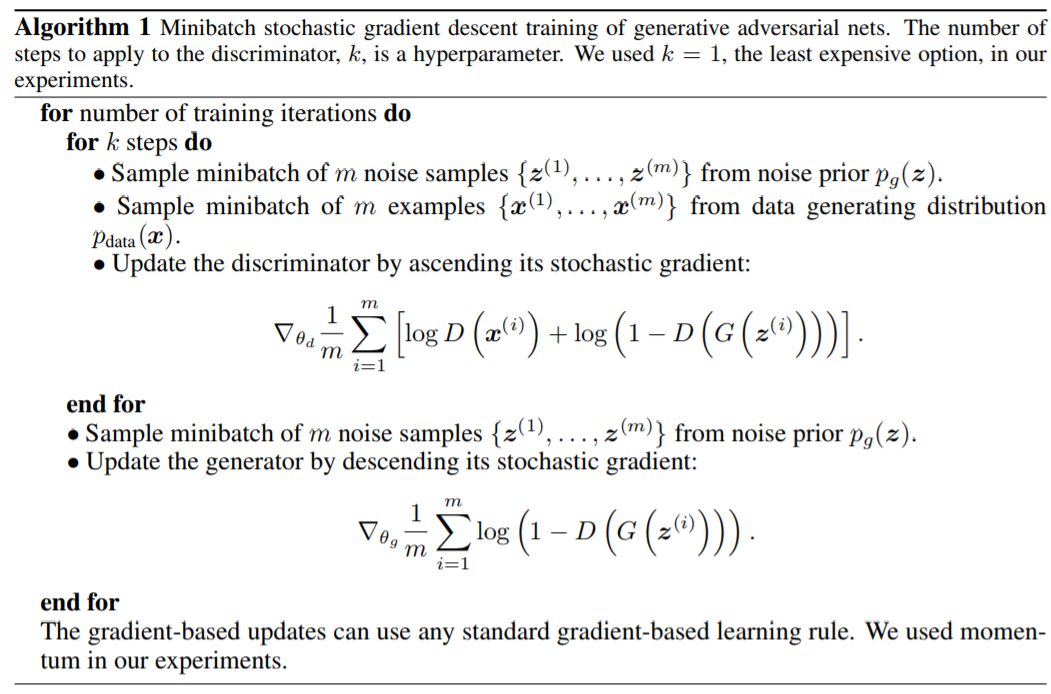
\includegraphics[width=\linewidth]{GAN-Goodfellow.PNG}
\caption{Algorithm description}
\end{figure}

\begin{equation}
\label{1.1}
D^{*}_{G}(x)=\frac{p_{data}(x)}{p_{data}(x)+p_g(x)} 
\end{equation}
\textbf{Theorem}. If \(p_{g}=p_{data}\) which means the global minimum. C(G) will achieve the value of $-log4$.

\section{Various GAN}
\subsection{MMGAN}
The one proposed by Goodfellow, the original loss function used for
 discriminator is $-log(1- D(x))$ (cross-entropy)

\subsection{NSGAN}
In NSGAN, the difference between it with MMGAN is that it starts to use $-log(D(x))$ because it proves that, at the begining, the gradient for $-log(1-D(x))$ is small which may not reasonable as we need the gradient to be large to converge. So with $log(D(x))$, it initialized a higher gradient at first and decreasing progressively.

\subsection{f-GAN}
First, it proves that every divergence can be represented by $D_f(P \mid Q)=\int_xq(x)f(\frac{p(x)}{q(x)})$, and $f$ function should comply two criteria: 1. convex function, 2. $f(1)=0$. When $f(x)=xlog(x)$, it is KL divergence, and if $f(x)=-log(x)$, it is reversed KL-divergence.

\textbf{Fenchel Conjugate}, it is saying that every f-divergence has a conjugate function which could also be optimized towards our objective. $f^*(t)=max(xt-f(x))$

A collection of f-divergence functions can be found here: \href{https://arxiv.org/pdf/1606.00709.pdf}{f-GAN: Training generative neural samples using variational divergence minimization}

In conclusion, choosing different f-divergence seems affect the results little.

\section{CGAN}
\subsection{Applications}
\subsection{Diagram}
\subsection{Loss Function}

\section{WGAN}

\subsection{Loss Function}
In WGAN, it tries to minimize the so called \textbf{Earth Movement} divergence. imagine two distribution $P$ and $Q$, now if we expect to move distribution $P$ towards $Q$, then how much effort should we put? This is exactly what we seek for minimizing.
\begin{figure}[H]
    \centering
    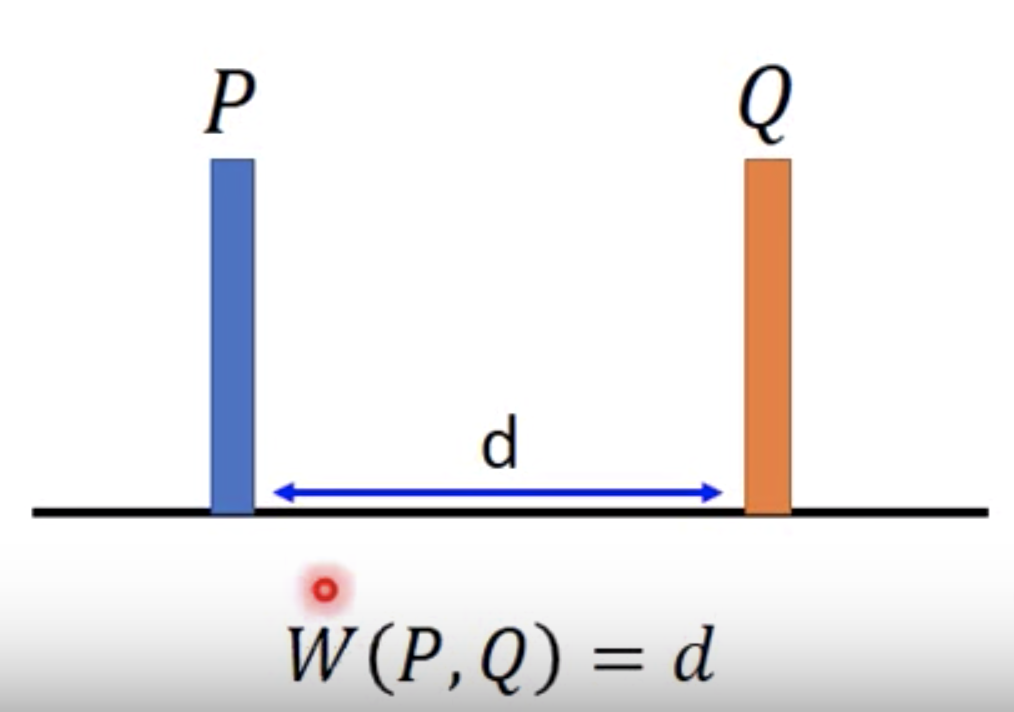
\includegraphics[width=200 pt]{W-GAN_loss}
    \caption{two distribution $P$ adn $Q$, the distance between $P$ and $Q$ is $d$. W-GAN is performing to minimize this $d$}
\end{figure}

According to the loss function, we should minimize the following equation:

\begin{equation}
    W(P_{data},P_G)=\max_{D\in 1-Lipschitz}\{E_{x \sim P_{data}}[D(x)]-E_{x \sim P_{G}}[D(x)]\}
\end{equation}

But, when applying gradient descent optimizer, it looks infeasible to force weights optimize with constraints "1-Lipschitz". Hence, the author proposed a method called "weight clipping". Put it simply, if weight larger than a threshold, then cut it becoming thaw-like.
\subsubsection{Generator loss}
\begin{figure}[H]
    \centering
    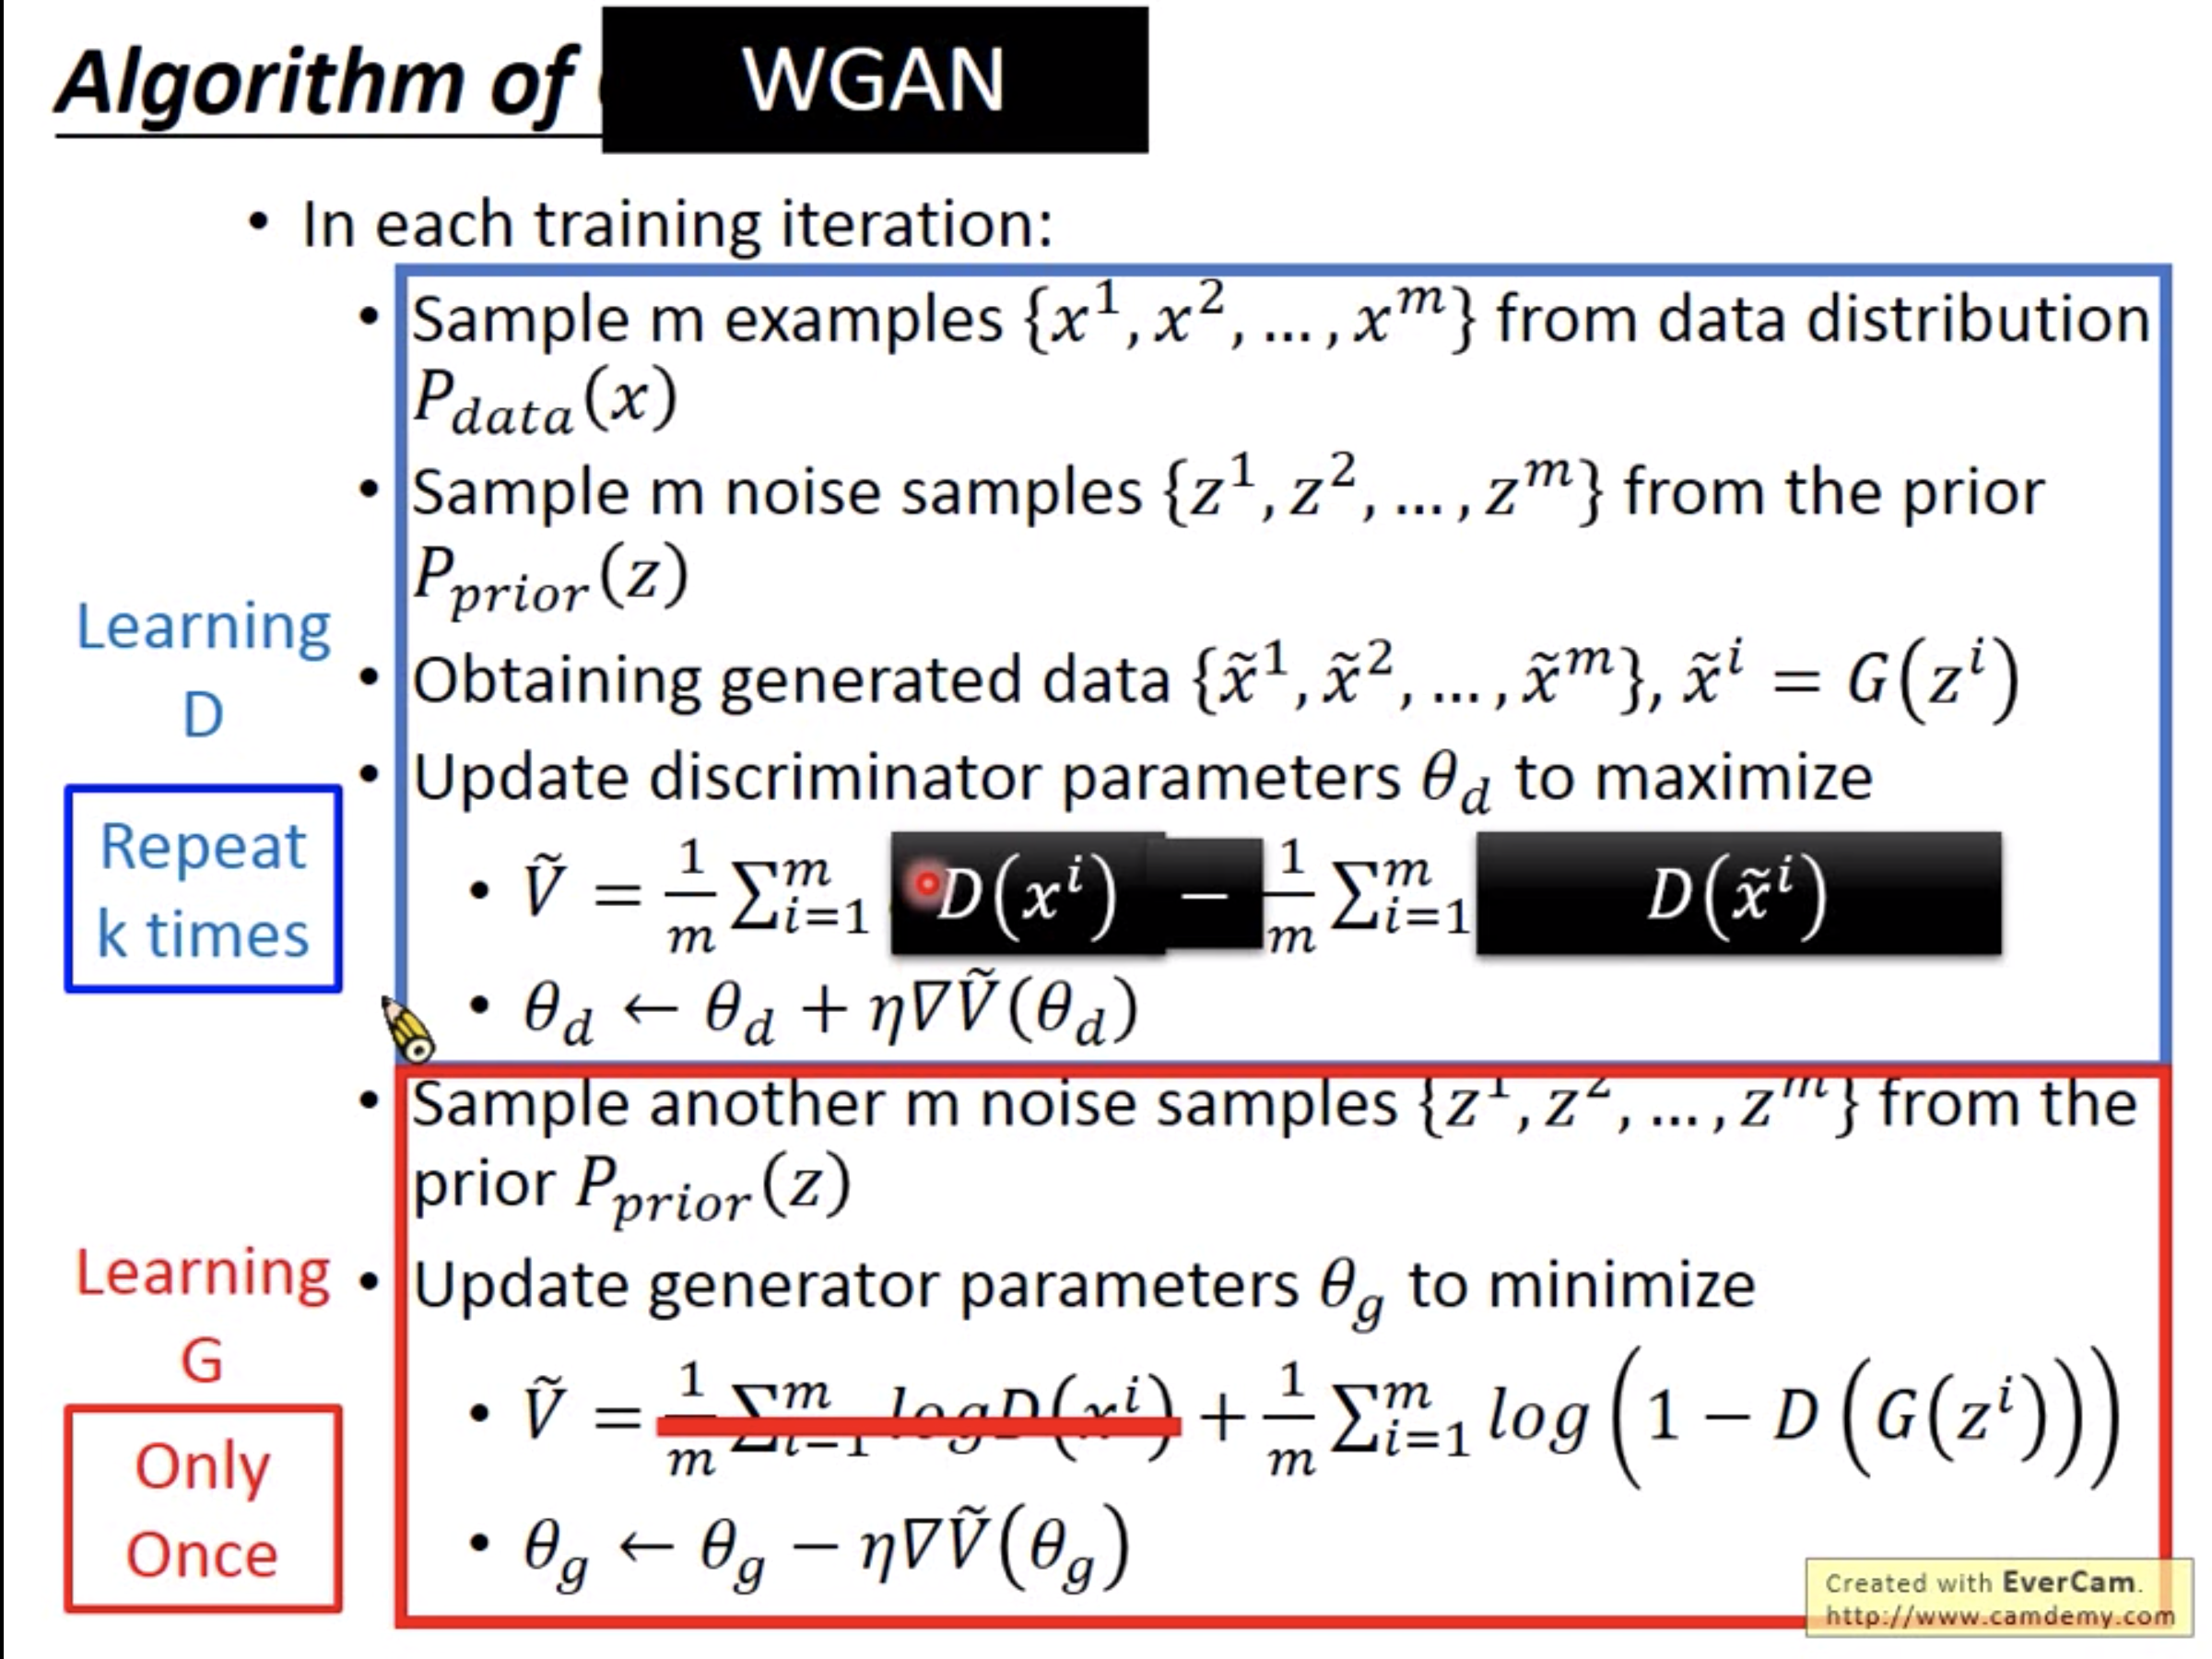
\includegraphics[width=\linewidth]{WGAN_algorithm}
    \caption{Description about WGAN}
\end{figure}


\section{improved WGAN}
\subsection{improvement compared to WGAN}
A differentiable 1-Lipschitz function if and only if it has gradient with norm less than or equal to 1 everywhere.

\begin{equation}
\begin{split}
    \mid \bigtriangledown_{x}D(x) \mid \leq 1  \\
    W(P_{data},P_G)=\max_{D} \{E_{x \sim P_{data}}[D(x)]-E_{x \sim P_{G}}[D(x)]- \lambda \sum_{x} \max(0, \mid \bigtriangledown_{x}D(x) \mid -1)dx \} \\
\end{split}
\end{equation}

it leverages an additional term "regularization" to satisfy the constrain that WGAN has proposed. But it is impossible to sample all x from that function. Instead, author decides to sample x from a penalty distribution. Then the equation becomes

\begin{equation}
    W(P_{data}, P_G)=\max_{D} \{ E_{x \sim P_{data}}[D(x)]-E_{x \sim P_{G}}[D(x)]- \lambda E_{x \sim Penalty}[max(0, \mid \bigtriangledown_{x} D(x) \mid -1)] \}
\end{equation}
\section{Energy-based GAN}
\subsection{difference}
\begin{itemize}
\item using auto-encoder as discriminator D\\
basically, it is saying that if an image feeding into discriminator, returns small reconstruction error, and then it proves this image is good.
\begin{figure}
    \centering
    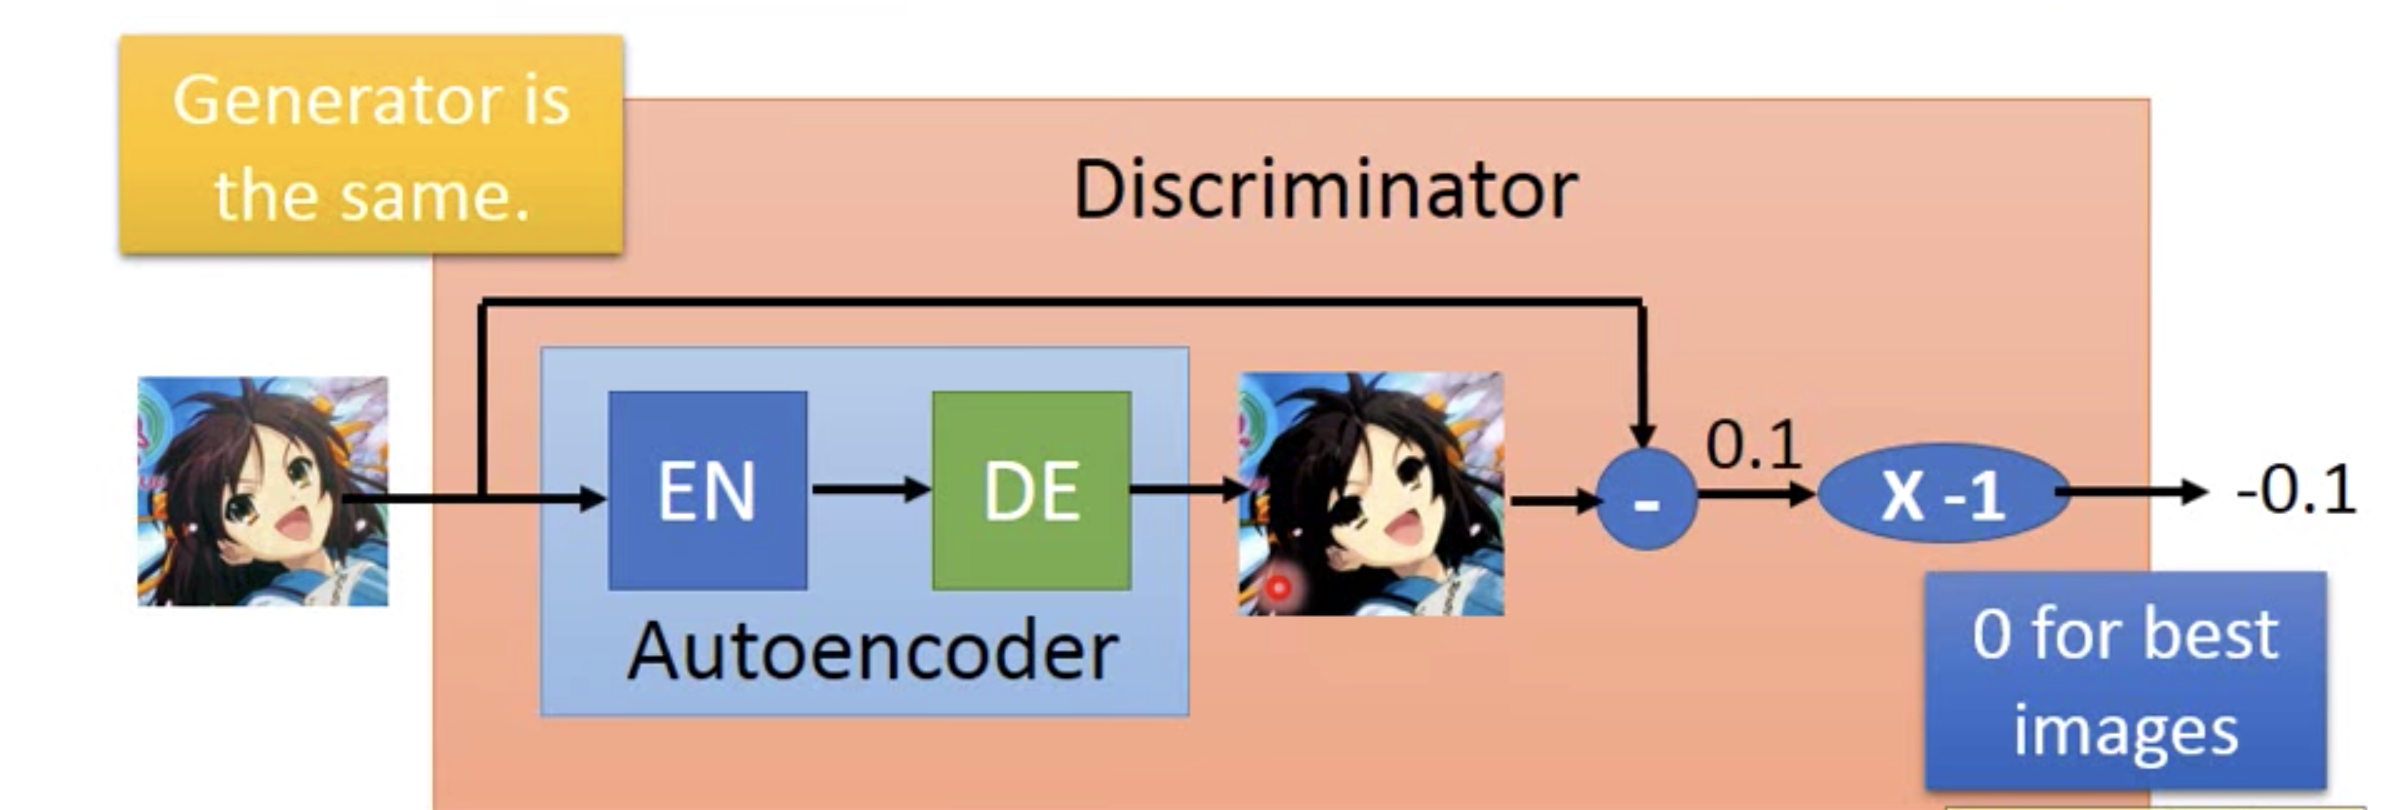
\includegraphics[width=\linewidth]{EBGAN}
    \caption{discriminator in EBGAN}
\end{figure}
\end{itemize}

\section{Divide and Conquer}
\subsection{Patch GAN}
Patch GAN is basically train the image by dividing it into sub-patches
\subsection{Stack GAN}
Stack GAN is used to generate high resolution image by creating multi-stages discriminator and generator. In the original paper, it intakes embedding texts and then in the first stage, generate 64x64 dimension images. After that, it creates 256x256 dimension in the second generator and discriminator.
\subsection{Progressive Growing GAN}
\begin{figure}[H]
    \centering
    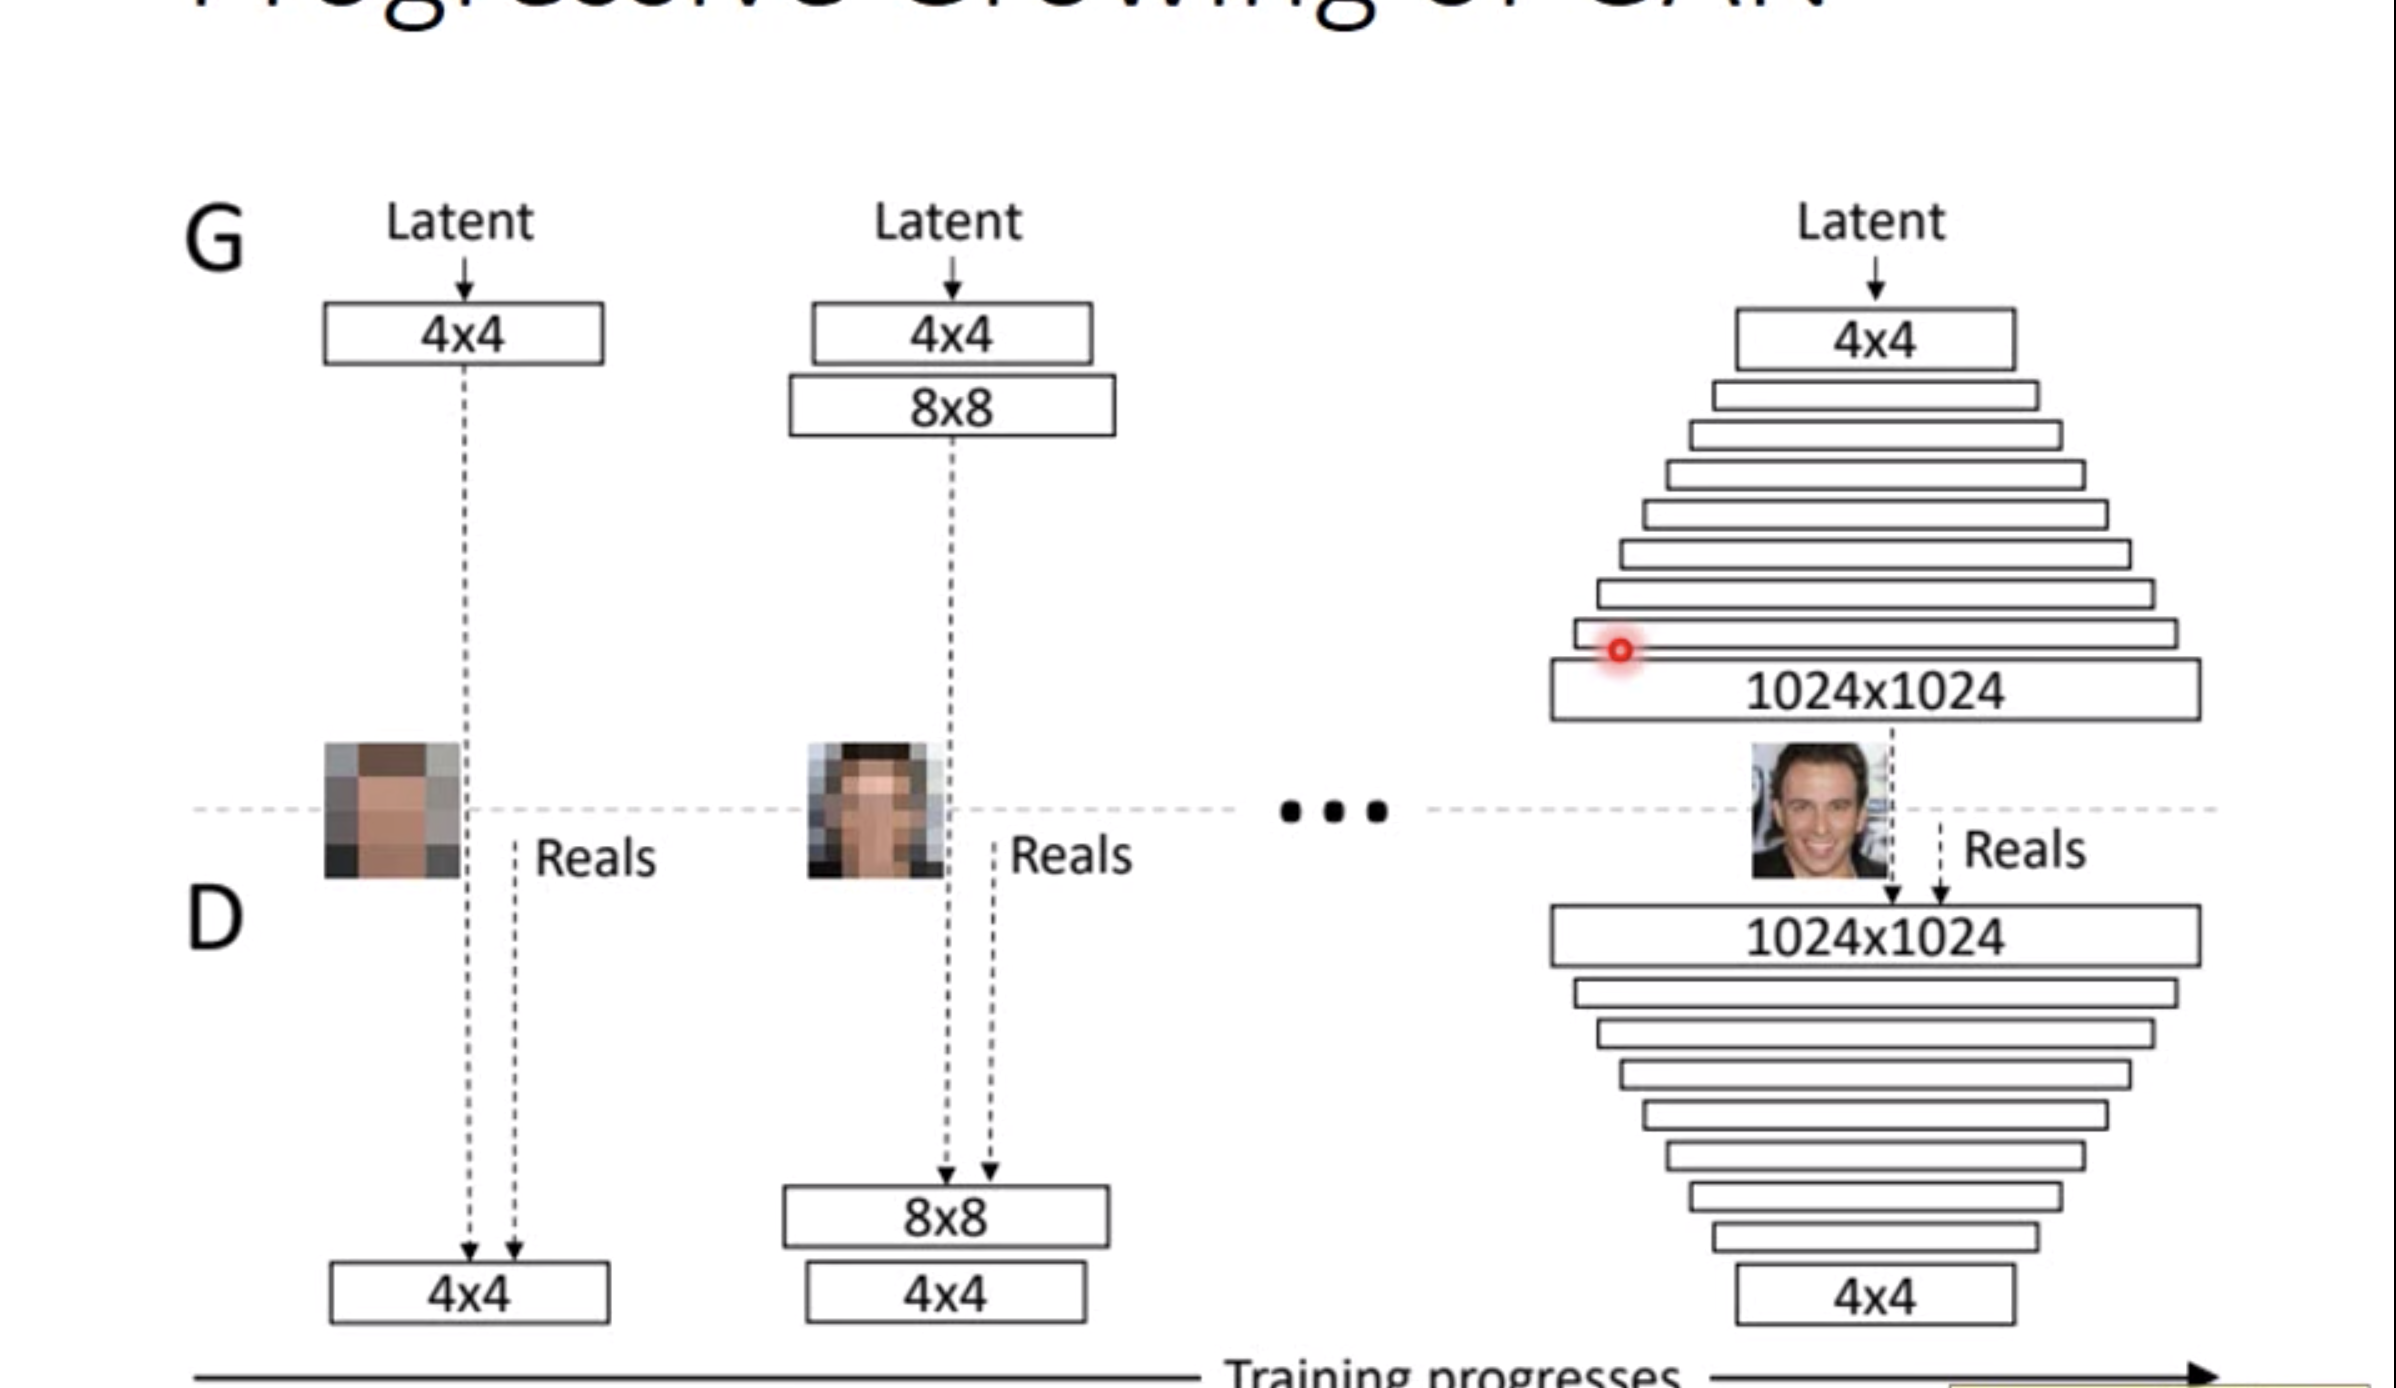
\includegraphics[width=\linewidth]{ProgressiveGAN}
    \caption{Progressive growing GAN}
\end{figure}
\section{SGAN}
\subsection{Applications}
\subsection{Diagram}
\subsection{Loss Function}
\subsubsection{Generator loss}
\section{infoGAN}
\subsection{Applications}
\textbf{infoGAN} could be used to control the image you want to generate. For instance, you can specify the input code to determine the digit to be bold/italic.
\subsection{Diagram}
\begin{figure}
    \centering
    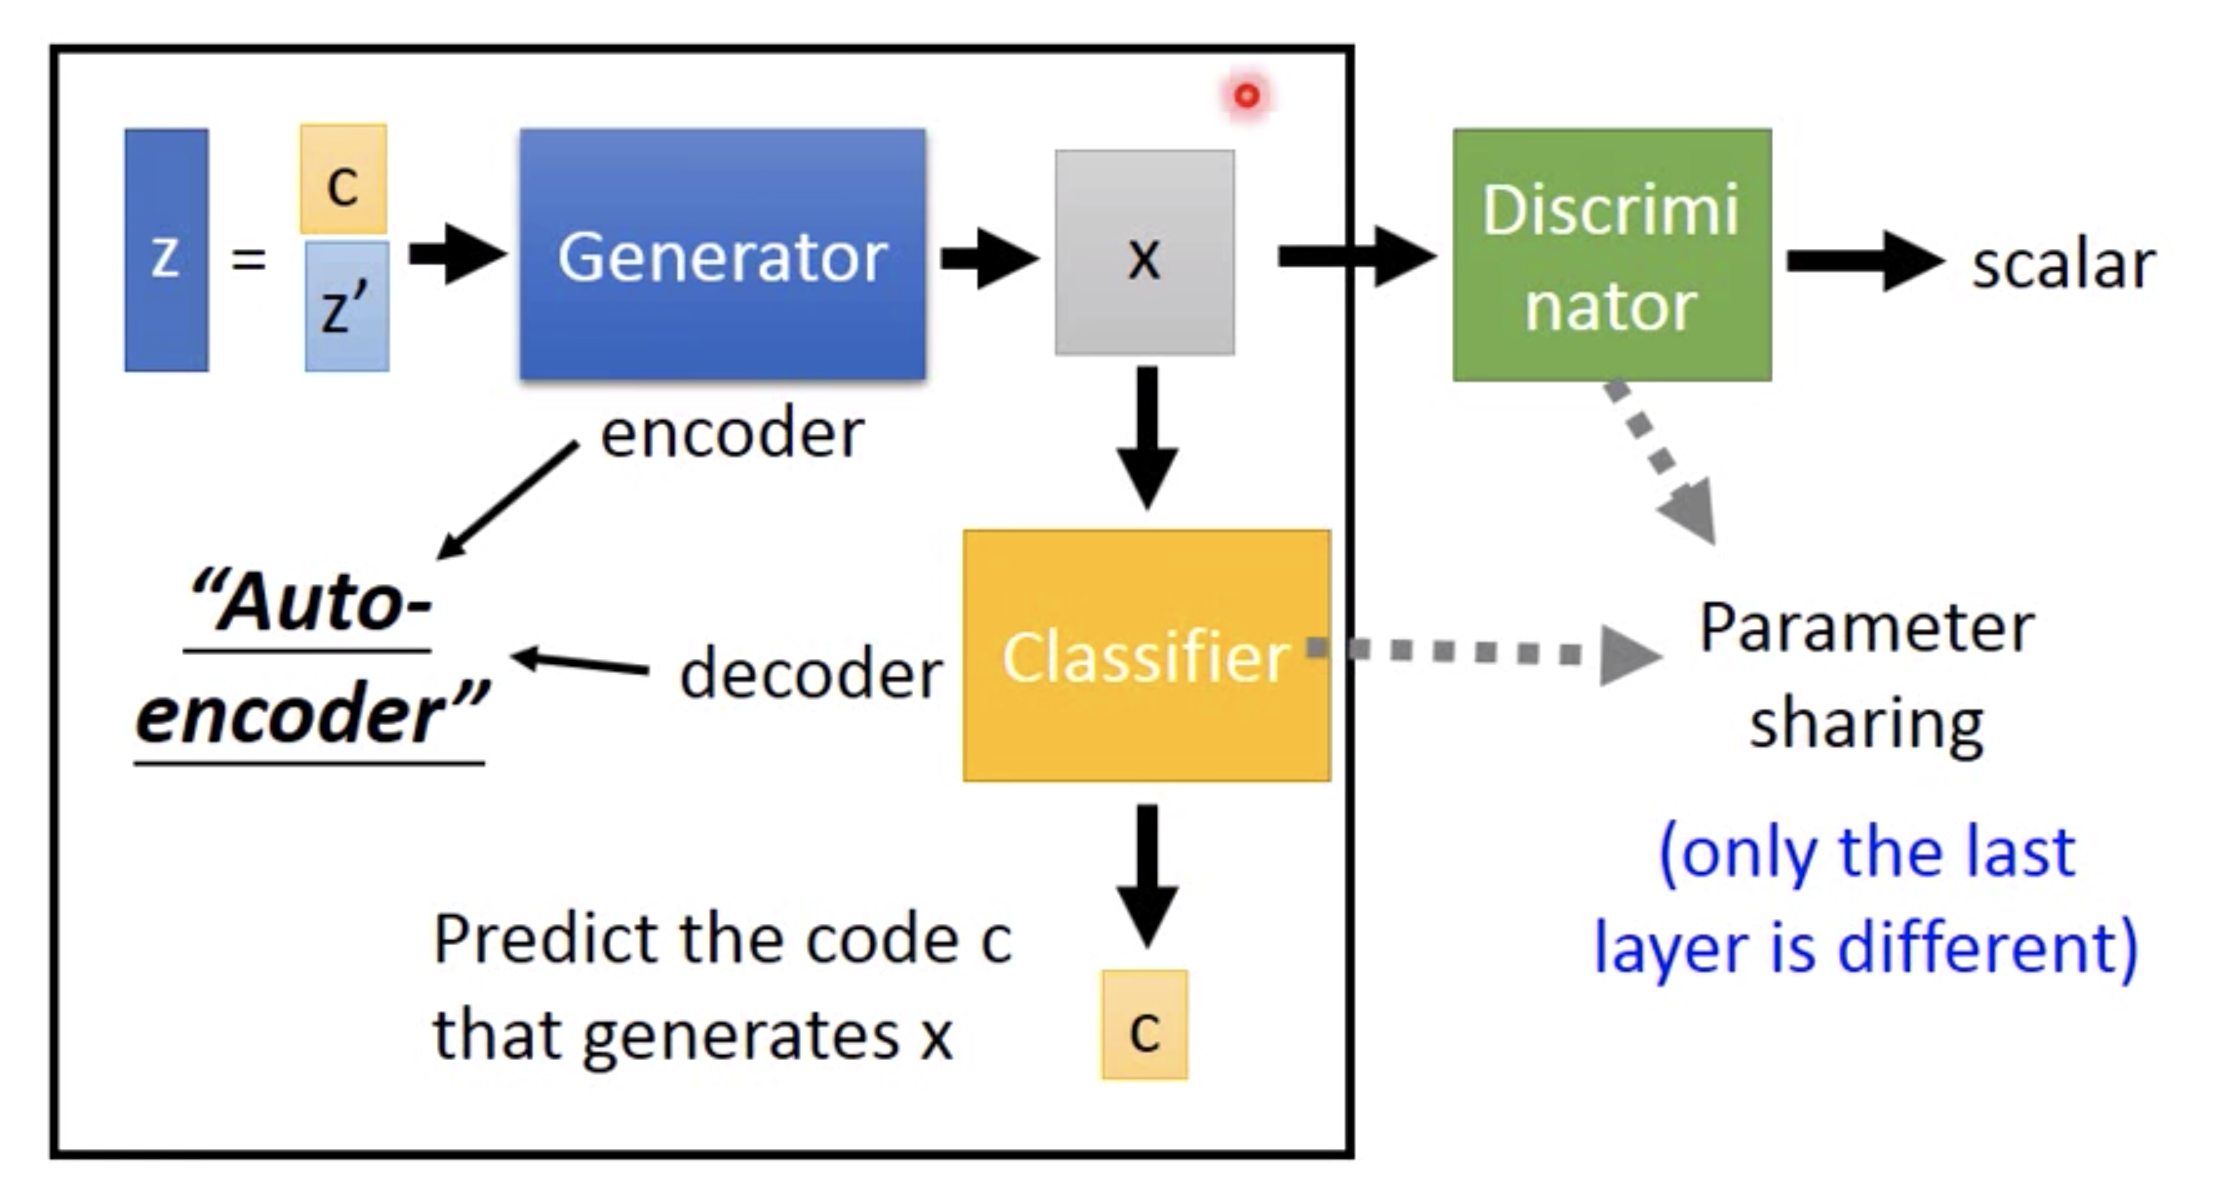
\includegraphics[width=\linewidth]{infoGAN}
    \caption{infoGAN}
\end{figure}
\section{Feature Disentangle}
\subsection{Applications}
\textbf{Feature disentangle} is used to generate the series variations for the object. For instance, we want to generate the face with different projections. That is to say, if you understand the feature within the code, then you can extract that feature, to generate something meaningful.
\section{Couple GAN}
\subsection{Applications}
Style Transfer
\subsection{diagram}
\begin{figure}[H]
    \centering
    \includegraphics[width=\linewidth]{coGAN}
    \caption{CoGAN}
\end{figure}
\section{UNIT: Unsupervised Image-to-image Translation}
\subsection{Applications}
image transfer, day-to-night,attribute based image translation, cat-to-cheetah.\href{https://github.com/mingyuliutw/UNIT}{github site}
\begin{figure}[H]
    \centering
    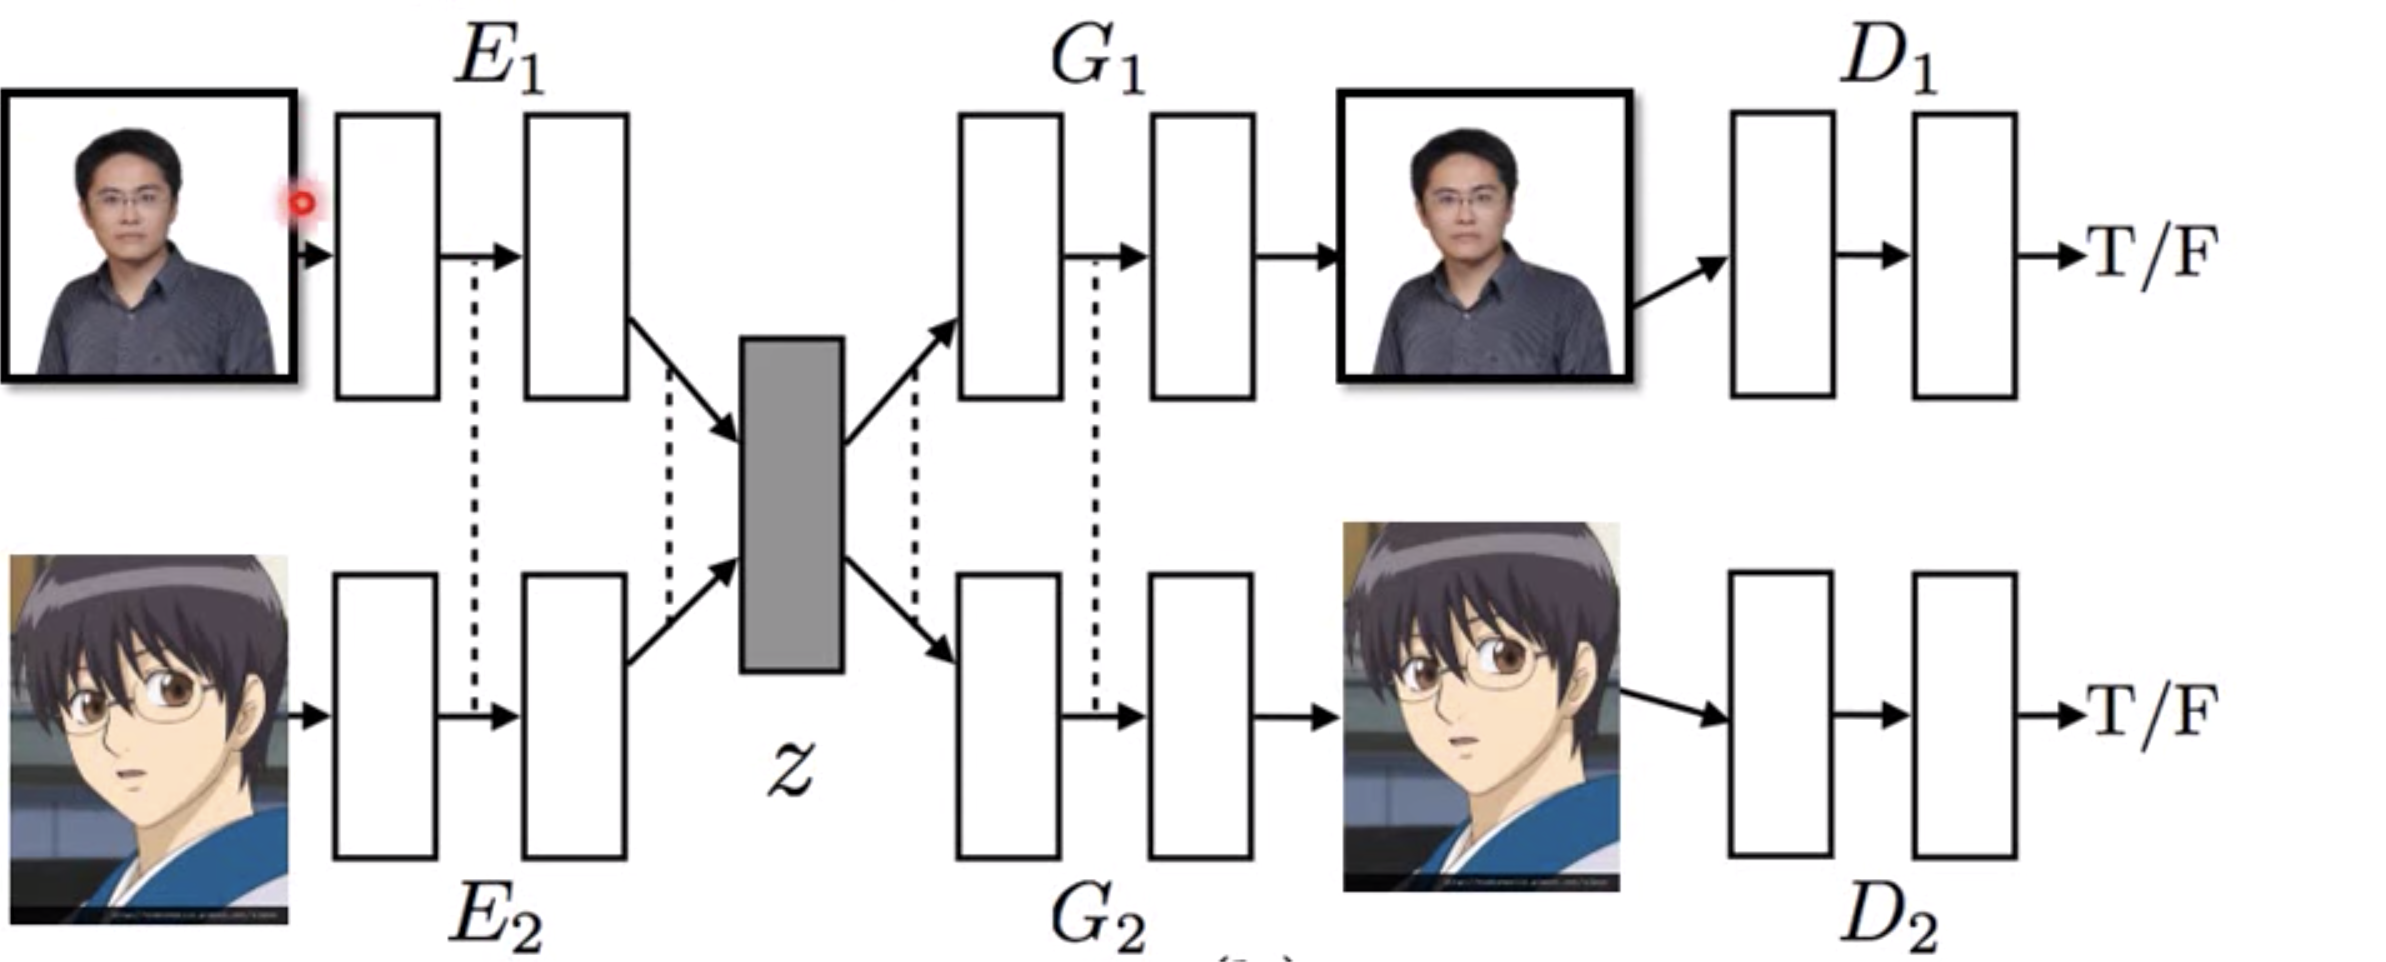
\includegraphics[width=\linewidth]{UNIT}
    \caption{UNIT}
\end{figure}
\section{tempoGAN}
\href{https://github.com/thunil/tempoGAN}{tempoGAN: A Temporally Coherent, Volumetric GAN for Super-resolution Fluid Flow}
\subsection{Applications}
It is one of the methods that have been coupling with traditional physics. In this paper, the author uses tempoGAN to generate super-resolution results from traditional fuilds simulation. Traditionally, 2D or 3D fluids model is constrained by the grid size. course grid may result in the numerical instability while fine grids of course wastes more time and may not feasible considering the equipment. But with the tempoGAN, we are able to generate high resolution fluids with less efforts.
\subsection{Key Points}
\begin{itemize}
\item first work to synthesize four-dimensional physics fields with neural networks
\item temporal discriminator
\item infer high resolution results with physical properties like velocity and vorticities.
\item Physical-aware data augmentation
\end{itemize}

\subsection{Diagram}
\begin{figure}[H]
\centering
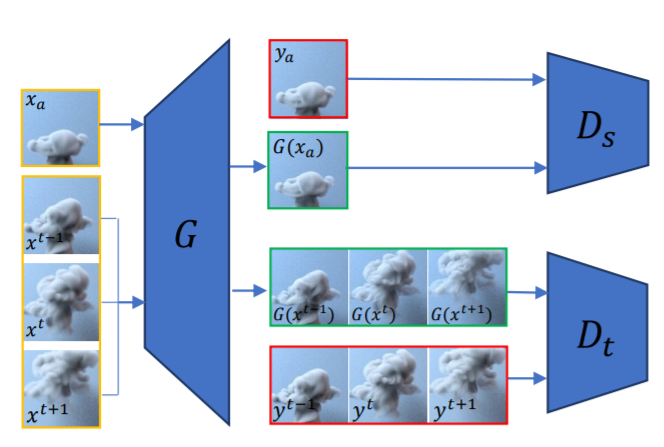
\includegraphics{tempoGAN_diagram}
\caption{schematic representation of tempoGAN framework}
\end{figure}
\subsection{Loss Function}
\subsubsection{Generator loss}
\section{Summary}
\begin{table*}[ht!]
\begin{tabular*}{\textwidth}{c @{\extracolsep{\fill}}|c|c|c}
\hline
GANS & Archive & Loss Function \\
\hline
GAN&\href{https://arxiv.org/pdf/1406.2661.pdf}{Arxiv}& $L_D^{GAN}=E[log(D(x))]+E[log(1-D(G(z))]$\linebreak$L_G^{GAN}=E[log(D(G(z)]$ \\

\hline
\end{tabular*}
\end{table*}
\end{document}
